\begin{figure}[!htb]
\begin{center}
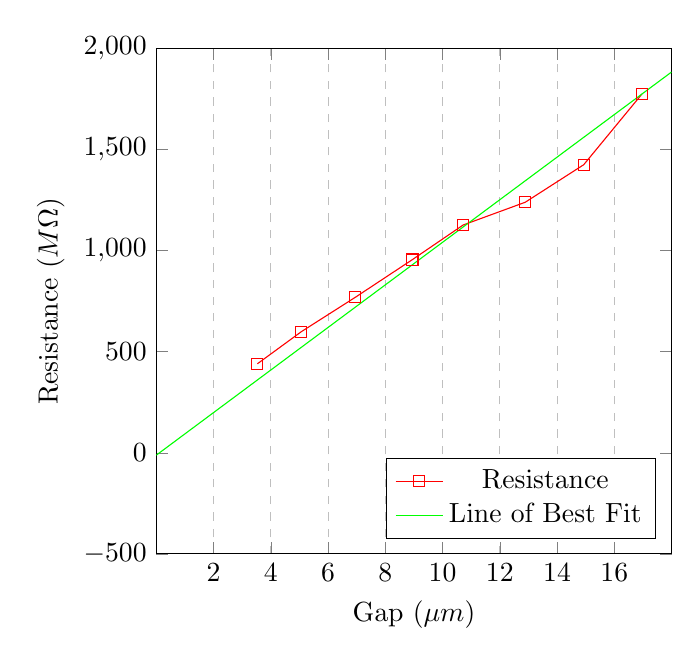
\begin{tikzpicture}

\begin{axis}[
    %title={Temperature dependence of CuSO$_4\cdot$5H$_2$O solubility},
    xlabel={Gap ($\mu m$)},
    ylabel={Resistance ($M\Omega$)},
    height=8cm,
    width=0.67\textwidth,
    xmin=0, xmax=18,
    ymin=-500, ymax=2000,
    xtick={2, 4, 6, 8, 10,12,14,16},
    ytick={-500, 0, 500, 1000, 1500, 2000},
    legend pos=south east,
    xmajorgrids=true,
    grid style=dashed,
]

\addplot[color=red, mark=square]
  coordinates {
    (3.5294, 440.302012013769)
    (5.0640, 599.1596921388986)
    (6.9493, 769.1633331672097)
    (8.9467, 955.8715312298274)
    (10.719, 1126.8803002926064)
    (12.887, 1239.3991541526978)
    (14.932, 1425.1543189284148)
    (16.966, 1774.7713800596902)
};
  \addlegendentry{Resistance}

% \addplot [
%   domain=0:18,
%   samples=100,
%   color=blue,
%     ]
%       {106.30760633430582*x - 43.05146906783261};
%       % \addlegendentry{Line of Best Fit using all data points}

\addplot [
  domain=0:18,
  samples=100,
  color=green,
    ]
    % {95.89874571698954*x + 80.29228665958908};
    {105.27516692493366*x - 11.327101988734285};
  % \addlegendentry{Line of Best Fit using $2-10\mu m$}
  \addlegendentry{Line of Best Fit}


\end{axis}
\end{tikzpicture}

\caption{Plot of Resistance vs TLM Gaps on Substrate A at $250\degree C$ with Line of Best Fit}
\label{fig:results:res_line_250}
\end{center}
\end{figure}
